\listfiles
\documentclass{article}
\author{Arya Stark}

\usepackage{amsmath}
\usepackage{amssymb}
\usepackage{mathtools}
\usepackage{listings}
\usepackage{float}
\usepackage{tikz}
\usepackage{tikz,fullpage}
\usepackage{tkz-graph}
\usepackage[position=top]{subfig}

\DeclarePairedDelimiter\floor{\lfloor}{\rfloor}
\DeclarePairedDelimiter\ceil{\lceil}{\rceil}
\DeclareMathOperator{\cl}{cl}
\DeclareMathOperator{\E}{E}
\def\Z{\mathbb{Z}}
\def\N{\mathbb{N}}
\def\R{\mathbb{R}}
\def\Q{\mathbb{Q}}
\def\K{\mathbb{K}}
\def\T{\mathbb{T}}
\def\B{\mathcal{B}}
\def\XX{\mathfrak{X}}
\def\YY{\mathfrak{Y}}
\def\AA{\mathfrak{A}}
\def\ZZ{\mathfrak{Z}}
\def\BB{\mathcal{B}}
\def\UU{\mathcal{U}}
\def\MM{\mathcal{M}}
\def\M{\mathfrak{M}}
\def\l{\lambda}
\def\L{\Lambda}
\def\<{\langle}
\def\>{\rangle}

\usepackage[a4paper,margin=1in]{geometry}

\setlength{\parindent}{0cm}
\setlength{\parskip}{1em}

\title{Virtual Channels and Rebalancing in State Channel Networks}
\date{}

\begin{document}
\maketitle

\section*{Introduction}

This research note was written because there are some unsolved problems in designing state channel networks that are not well-known or being worked on. Precisely defining these problems requires formally modelling of state channel networks, and the problems presented are only present if the formal models include agents' preferences over network topology (payment capacity), blockchain fees, and capital costs.

\section*{Relevant Prerequisite Literature}

This section goes through relevant existing literature. Note that even if you know all this, many definitions will be used in later sections.

\subsection*{Ball-and-bead model of PCN}

I first saw this nice model from Peter Rizun on Twitter. TBW.

\subsection*{Rebalancing}

We say that two channel networks are value-equivalent if the set of agents is the same and each agent owns the same. A channel network is rebalanced when it transitions into a value-equivalent state. This transition can include on-chain transactions or not. Here are examples.

In the ball-and-bead model, an on-chain rebalance is represented by "hopping wires".

Are off-chain rebalances sufficient? In general, no. In fact we can import the existing literature on flow networks to state this quite precisely.

TBW: define a $a,b$-flow, apply max-flow-min-cut theorem, etc.

Note some assumptions implicitly made when applying this theorem: the max flow might requrie very global knowledge to compute.

Fun exercise! A self-payment is a special type of off-chain rebalance. Show that any rebalance can be expressed as a series of self-payments.

\subsection*{Subchannels}

Also known as channel factories, although this is not such a good name.

\subsection*{Virtual Channels}

TBW

\subsection*{State Channel Networks}

\subsection*{Multipath}

\subsection*{Ejecting Virtual Channels}

\subsection*{Plasma}

Claim: a super-optimized channel network will be less useful than a very suboptimal one that supports funding via plasma!

\section*{Informal Formal Model}

\section*{Ejection Test Cases}

\subsection*{Asymetric}

\begin{figure}[H]
    \centering
    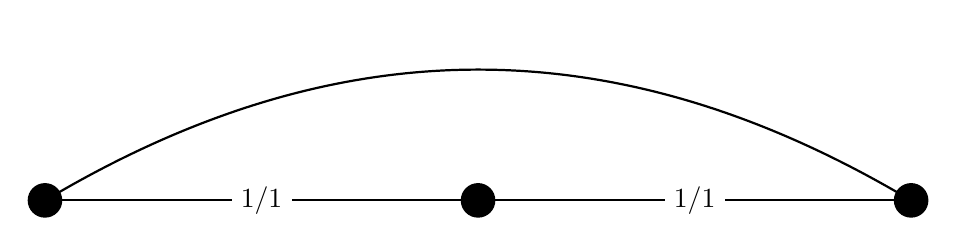
\begin{tikzpicture}[scale=2.75]
        \GraphInit[vstyle=Normal]
        \SetVertexSimple
        \Vertex[x=0,y=0]{A}
        \Vertex[x=2,y=0]{B}
        \Vertex[x=4,y=0]{C}
        \Edge[label=$1/1$](A)(B)
        \Edge[label=$1/1$](B)(C)
        \Edge[style={bend left}](A)(C)
    \end{tikzpicture}
    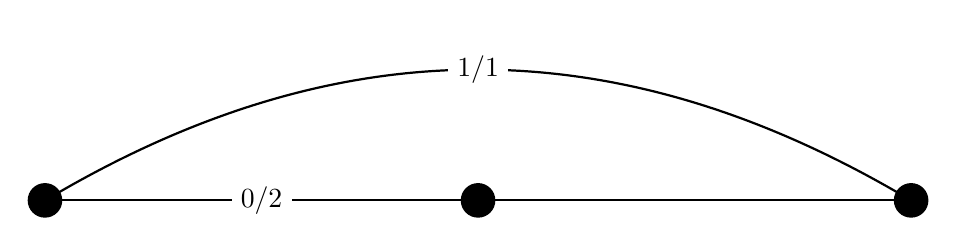
\begin{tikzpicture}[scale=2.75]
        \GraphInit[vstyle=Normal]
        \SetVertexSimple
        \Vertex[x=0,y=0]{A}
        \Vertex[x=2,y=0]{B}
        \Vertex[x=4,y=0]{C}
        \Edge[label=$0/2$](A)(B)
        \Edge(B)(C)
        \Edge[style={bend left},label=$1/1$](A)(C)
    \end{tikzpicture}
\end{figure}

This manner of ejectning might be preferred because it minimal in the number of transactions. Even after account abstraction, it is minimal in the number of ERCECOVERS.

\subsection*{Symmetric}

\begin{figure}[H]
    \centering
    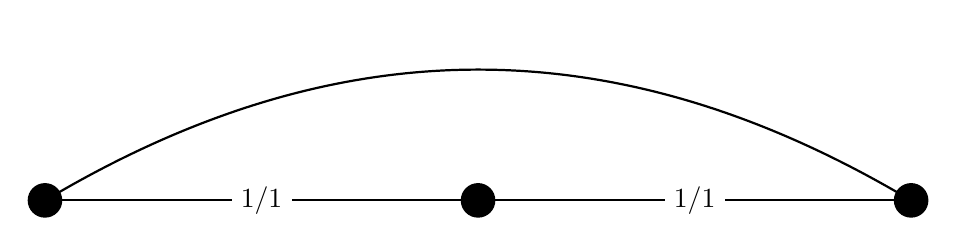
\begin{tikzpicture}[scale=2.75]
        \GraphInit[vstyle=Normal]
        \SetVertexSimple
        \Vertex[x=0,y=0]{A}
        \Vertex[x=2,y=0]{B}
        \Vertex[x=4,y=0]{C}
        \Edge[label=$1/1$](A)(B)
        \Edge[label=$1/1$](B)(C)
        \Edge[style={bend left}](A)(C)
    \end{tikzpicture}
    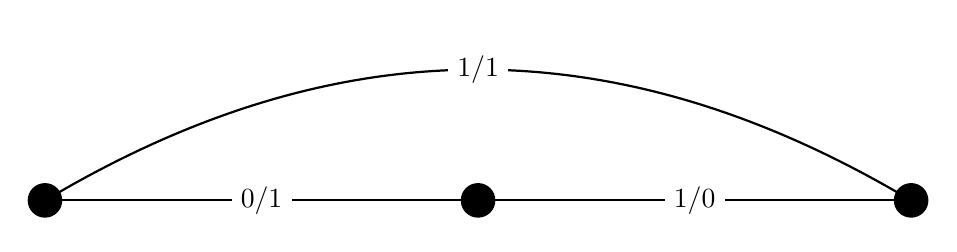
\begin{tikzpicture}[scale=2.75]
        \GraphInit[vstyle=Normal]
        \SetVertexSimple
        \Vertex[x=0,y=0]{A}
        \Vertex[x=2,y=0]{B}
        \Vertex[x=4,y=0]{C}
        \Edge[label=$0/1$](A)(B)
        \Edge[label=$1/0$](B)(C)
        \Edge[style={bend left},label=$1/1$](A)(C)
    \end{tikzpicture}
\end{figure}

Might be preferred because of capacity

\subsection*{Symmetric Unidirectional}
\subsection*{Asymmetric Unidirectional}

\subsection*{Long-Chain Large-Radius}
\subsection*{Long-Chain Short-Radius}
\subsection*{Multipath}
\subsection*{Long-Chain Multipath}
\subsection*{Thanos Star}

Minimal in number of transactions

\subsection*{Self-Lock-In}






\end{document}